\documentclass[../main.tex]{subfiles}
\graphicspath{{\subfix{../images/}}}
\begin{document}

  % Precisamos agrupar melhor esses testes, dar uma logica e introduzir
  Os testes seguiram a ordem e atenderam às especificações apresentadas na metodologia. Os resultados serão apresentados a seguir.

  \subsection{Cinemática Inversa}

  A partir das equações obtidas para a Cinemática Inversa do robô, o sistema é capaz não só de realizar a cinemática de cada uma das pernas individualmente, como também do seu corpo em todos os 6 graus de liberdade (translações em $x, y, z$ e rotações em $roll, pitch, yaw$). A figura \ref{fig:moving_body} ilustra o movimento do corpo do robô em cada um desses graus de liberdade.

  \begin{figure}[h]
    \centering
    \caption{Titulo da Figura}
    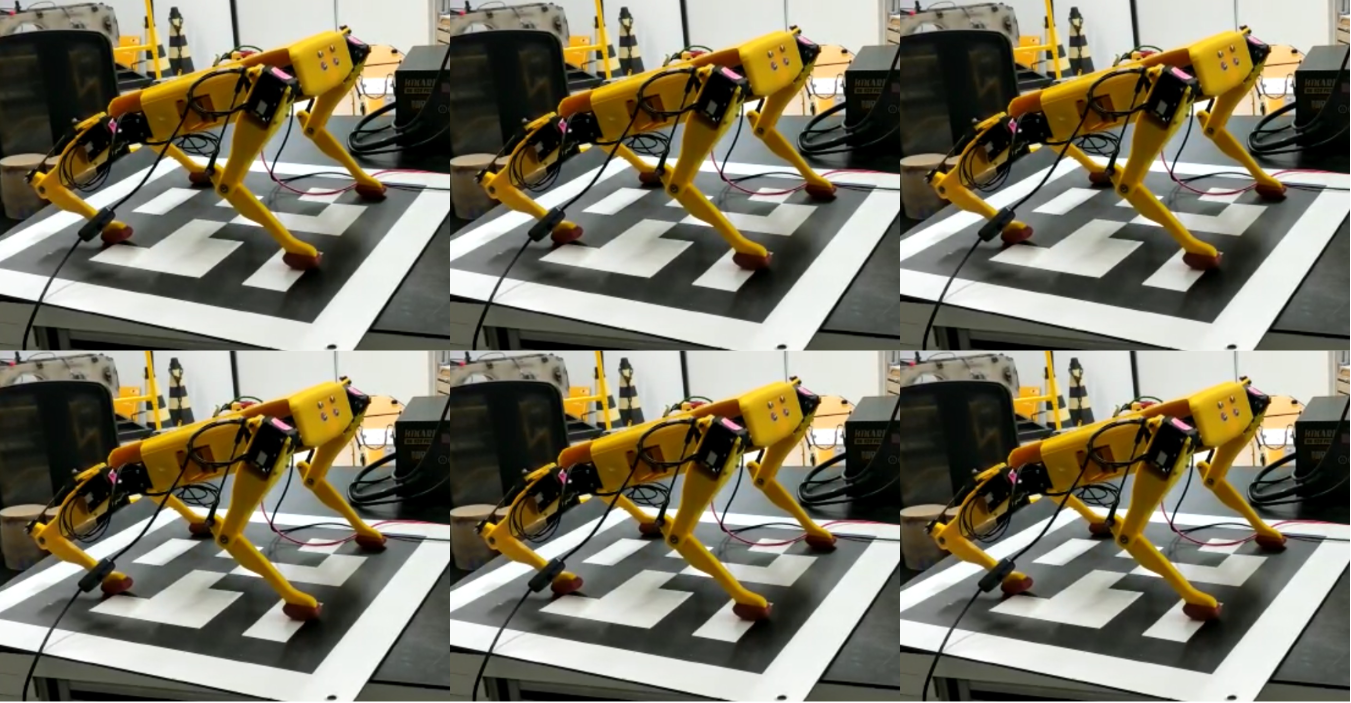
\includegraphics[width=0.48\textwidth]{moving_body.png}
    
    Fonte: XXX
    \label{fig:moving_body}
  \end{figure}

  \subsection{Controle de Rotação}

  Os gráficos da figura \ref{fig:grafico_controlling} ilustram o comportamento do sistema à variação dos \textit{setpoints} de orientação em $X$ (gráfico superior) e em $Y$ (gráfico inferior) para o corpo do robô, a partir da aplicação de diversos degraus (em azul). Nota-se que o protótipo é capaz de se adaptar rapidamente aos novos valores desejados de orientação, simultaneamente em ambos os eixos.

  \begin{figure}[h]
    \centering
    \caption{Titulo da Figura}
    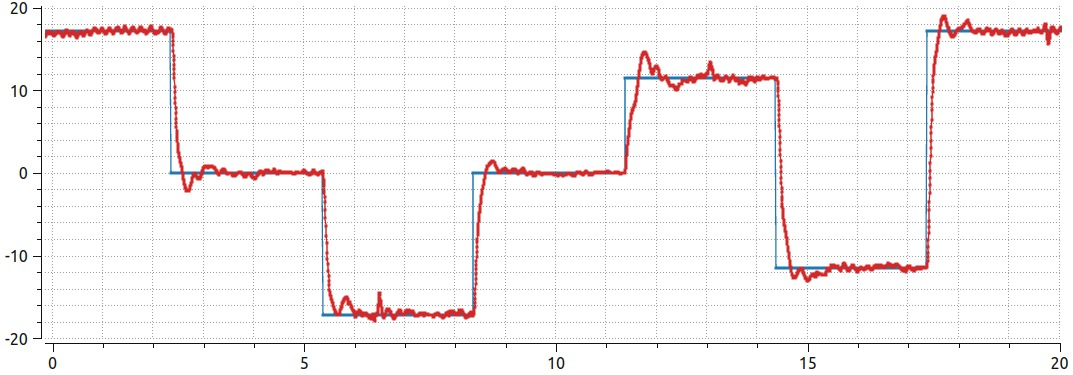
\includegraphics[width=0.48\textwidth]{grafico_controlling_X.png}
    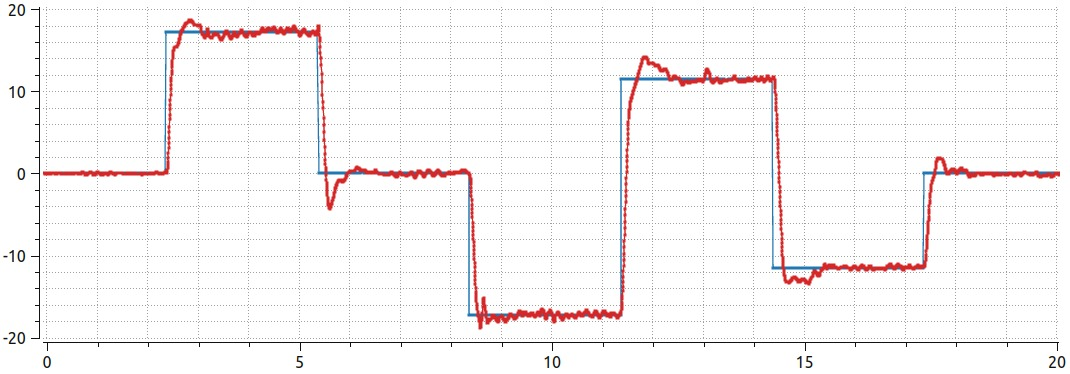
\includegraphics[width=0.48\textwidth]{grafico_controlling_Y.png}
    
    Fonte: XXX
    \label{fig:grafico_controlling}
  \end{figure}

  \subsection{Análise de trajetória}
  Durante este experimento, o corpo do protótipo está estático e suspenso por um suporte, sendo solicitado que uma de suas patas realize duas trajetórias calculadas pelo algoritimo proposto. Para geração das trajetórias foi considerado um período de $0.5 s$, altura do passo de $0.05 m$ e resolução de 25 pontos com distribuição homogênea, com deslocamentos em $(x, y)$ de $(0.05, 0.03)$ e $(0.03, 0.05)$ respectivamente, sendo realizados 30 testes para cada caso. 
  
  O objetivo aqui é analisar o tempo real de execução da trajetória, as coordenadas finais $(x_f, y_f)$ da pata e a altura máxima $z_{max}$ atingida durante o passo, comparando-os com os valores desejados para cada um desses parâmetros. A tabela \ref{tab:trajetoria} traz as médias encontradas para cada um desses parâmetros durante a realização dos testes.

  \begin{table}[h]
    \caption{Titulo da Tabela}
    \centering
      \begin{tabular}{lllll}
             & $tempo (s)$ & $x_{final}(m)$ & $y_{final}(m)$ & $z_{max}(m)$ \\
      Exp. 1 & 0.559457 & 0.050349 & 0.029247 & 0.047585 \\
      Exp. 2 & 0.556770 & 0.030240 & 0.049132 & 0.046562      
      \end{tabular}

    Fonte: Autoria própria
    \label{tab:trajetoria}
  \end{table}

  Inicialmente, foram realizados dois testes de T Student para amostras independentes, o primeiro relacionando o tempo de execução da trajetória nos experimentos 1 e 2, e o segundo relacionando a altura máxima alcançada, com o intuito de verificar se os resultados se alteram para diferentes valores $(x, y)$ desejados. O resultado da análise de T Student traz um $t$ de aproximadamente $1.087$, em se tratando de tempo, e de $1.0658$ para a altura máxima alcançada durante o passo. Para uma confiabilidade de $95\%$ e um total de 58 graus de liberdade, o valor crítico $t_c$ encontrado é de $2.00$. Como ambos os valores encontrados estão dentro do intervalo de confiança ($-t_c < t < t_c$), isso mostra que não há uma diferença significativa entre as médias em cada experimento, o que significa que diferentes comandos de trajetórias em $(x, y)$ não interferem nos resultados de tempo e altura máxima do passo.
  
  Os gráficos da figura \ref{fig:grafico_trajetoria_xyz} representam um dos testes realizados para o primeiro caso ($x=0.05m$, $y=0.03m$), sendo os gráficos superiores esquerdo e direito correspondentes à trajetória em $x$ e $y$ respectivamente, e o gráfico inferior correspondente à trajetória em $z$ (altura do passo). Nota-se que, como esperado pela análise da tabela \ref{tab:trajetoria}, há um atraso na execução da trajetória (neste caso específico de aproximadamente $54ms$) e a altura máxima alcançada é levemente inferior à desejada (alcançando neste caso um valor próximo a $0.0476m$).

  \begin{figure}[h]
    \centering
    \caption{Titulo da Figura}
    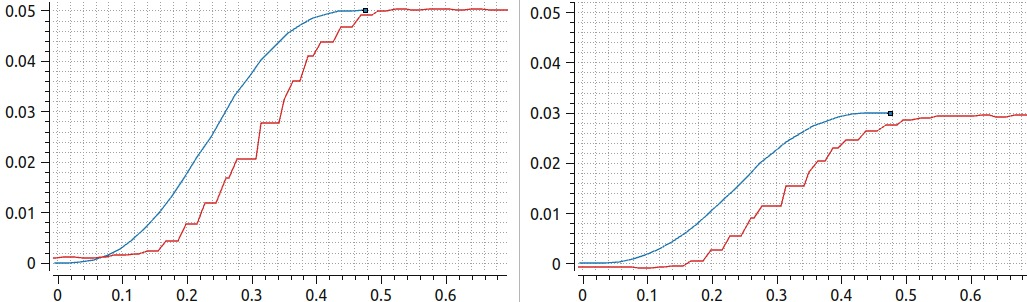
\includegraphics[width=0.48\textwidth]{grafico_trajetoria_xy.png}
    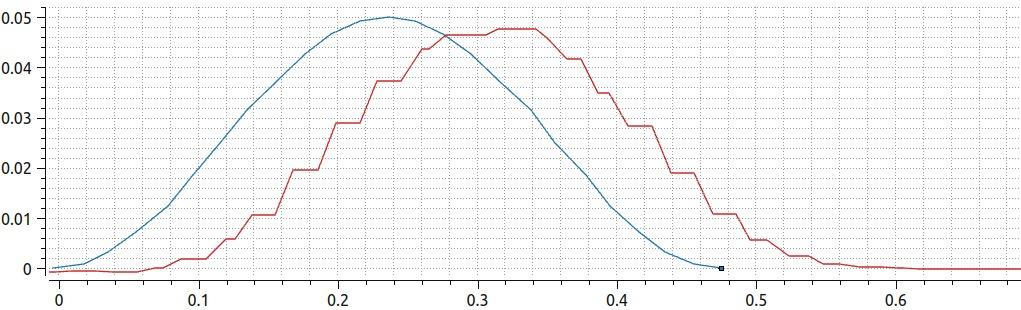
\includegraphics[width=0.48\textwidth]{grafico_trajetoria_z.png}
    
    Fonte: XXX
    \label{fig:grafico_trajetoria_xyz}
  \end{figure}

  \subsection{Controle de velocidade}
  Durante os testes de controle de velocidade, de maneira geral, foi observado uma caminhada eficiente em ambos os terrenos, porém, mais linear e com menor trepidação em terrenos planos do que em terrenos irregulares. Por meio dos dados coletados, foram extraídos as informações, velocidade média da caminhada, oscilação máxima de rotação do corpo em roll e pitch e os respectivos desvios padões, e apresentados na Tabela \ref{tab:vel_stab}. Assim, foi observado que a menor oscilação em roll e em pitch ocorreu no terreno plano utilizando o controle de rotação, enquanto que a maior ocorreu nas condições opostas (teste 3).  Por outro lado, o robô se aproximou mais vezes da velocidade solicitada no terreno plano combinado ao controle de rotação, enquanto que no irregular com controle de rotação foi apresentada uma velocidade média inferior e baixa consistência nos dados.

  \begin{table}[]
    \caption{Titulo da Figura}
    \centering
    \begin{tabular}{ccccc}
      \hline
      & 1 & 2 & 3 & 4 \\ \hline
      Terreno & Reg. & Reg. & Irreg. & Irreg. \\ \hline
      \begin{tabular}[c]{@{}c@{}}C. R.\end{tabular} & Não & Sim & Não & Sim \\ \hline
      \begin{tabular}[c]{@{}c@{}}Vel. \\(m/s)\end{tabular} & 0.0292 & 0.0333 & 0.0297 & 0.0277 \\ \hline
      \begin{tabular}[c]{@{}c@{}} $\sigma_{Vel}$  \end{tabular} & 0.00135 & 0.00079 & 0.00197 & 0.00241 \\ \hline
      \begin{tabular}[c]{@{}c@{}} $\Delta_{Roll}$ \end{tabular} & 12.541 & 8.742 & 13.897 & 12.168 \\\hline
      \begin{tabular}[c]{@{}c@{}} $\sigma_{Roll}$ \end{tabular}  & 2.416 & 2.145 & 1.802 & 3.270 \\ \hline
      \begin{tabular}[c]{@{}c@{}} $\Delta_{Pitch}$ \end{tabular} & 11.458 & 8.295 & 15.189 & 13.182 \\ \hline
      \begin{tabular}[c]{@{}c@{}} $\sigma_{Pitch}$ \end{tabular}  & 1.826 & 2.386 & 1.441 & 2.944 \\ \hline

    \end{tabular}
    Fonte: Autoria própria
    \label{tab:vel_stab}
  \end{table}

  A fim de avaliar se o controle de rotação aqui proposto contribuiu de fato na estabilidade da caminhada, utilizaremos o teste T-Student de uma amostra, com um nível de confiança de 99\%. Então, foi proposto que a hipotése nula é que a oscilação de rotação do corpo não foi melhorada com o uso do controle de rotação, considerando testes entre os mesmos terrenos. O resultado desta análise nos mostrou que a hipotése nula pode ser rejeitada, uma vez que os valores t-crítico para uma calda foram maiores que 0.01. Logo, pode-se afirmar que quando utilizado o controle de rotação é observado uma caminhada mais estável.
  
  %% Sugiro juntar essas section em uma só, pra economizar espaço
  \subsection{Plano inclinado}
  Durante este experimento, contatou-se que o robô possui a habilidade de andar por terrenos com até 5,336\degree de inclinação. Entretanto, foi observado uma melhor estabilidade em inclinações de até X\degree. 
  
  \subsection{Superação de obstáculos}
  O Caramelo se mostrou capaz de ultrapassar obstáculos de até 5cm de altura. 

  COLOCAR UMA IMAGEM DOS DOIS TESTES JUNTAS A e B

  TABELA DE ANALISE T-STUDENT PRA COLOCAR NO APENDICE 



   


\end{document}